\chapter{Evaluation} \label{EvaluationChapter}

In this chapter, we describe our approach to evaluating the new cloud-based execution environment in terms of performance, operating costs, as well as benefits brought to the end user. We describe the results of various benchmarks run against clusters with different configurations and discuss the challenges involved in correctly identifying the most influencing factors for the performance of distributed systems.

Although the specific end goal of the project was providing a new environment for running experiments on AWS from OpenMOLE, we also benchmark the underlying GridScale AWS module separately, since it can be used as a standalone component. We use DoC's\footnote{Imperial College's Department of Computing} HTCondor and Slurm deployments to compare the speed of the new system with a locally hosted cluster.

Throughout the chapter, we delve into considerations about the costs of running specific workflows on AWS and advocate the use of different types of clusters depending on the nature of the workload. To illustrate the benefits of the fully automated job delegation to the cloud, we contrast it with the manual steps previously needed to obtain similar results with other experiment frameworks.

\section{Fully Automated Experiments}

OpenMOLE is now, to our knowledge, the only scientific experimentation framework that allows users to run experiments on commercial cloud environments without any form of configuration beyond providing their credentials. Listing \ref{EnvSwitch} shows how the switch to the cloud is made by injecting the new environment in the workflow instantiation.

\begin{listing}[h]
	\centering
	\begin{minipage}{11.6cm}
		\begin{minted}[frame=single,framesep=2mm,escapeinside=||,baselinestretch=1.15,fontsize=\small,linenos]{scala}
val (t1, t2, t3) = (EmptyTask(), EmptyTask(), EmptyTask())
		
val localhost = LocalEnvironment(threads = 8)
val aws = AWSEnvironment(
  region = "eu-west-1",
  awsUserName = "adrian",
  awsUserId = "434676269080",
  awsKeypairName = "gridscale",
  awsCredentialsPath = "/Users/adrian/.aws/credentials.csv",
  privateKeyPath = "/Users/adrian/.ssh/id_rsa",
  clusterSize = 8
)

val localMole = t1 -- (t2 on localhost) -- t3
val cloudMole = t1 -- (t2 on aws) -- t3
		\end{minted}
	\end{minipage}
	\caption{Creating an experiment ready to run both locally an in the cloud.}
	\label{EnvSwitch}
\end{listing}

As described in the background chapter, other workflow platforms such as Taverna, Galaxy, or the Humman Connectome project have recently started cloud initiatives, but they still rely on a tedious setup on behalf of the user, who is required to follow long and complicated instruction steps \cite{TavernaAWS, GalaxyAWS, Connectome}. 

Although quantifying the ease of use is a subtle task, we have so far been encouraged by feedback. We believe that features such as automatically mapping resources to cloud instances and generating bidding strategies for spot instances bring a quality of life improvement and encourage more users to take advantage of commercial clouds for research.

\section{GridScale Benchmarks}

As the foundation layer OpenMOLE's access to remote resources, GridScale bears significant importance for the overall performance of the application. We believe that benchmarks at this level offer valuable insights into the impact of choosing an appropriate instance type for the master node of the cluster, since the job submission system is evaluated in isolation from other configuration and setup routines employed by higher level systems.

\subsection{Methodology}

In this section, we particularly focus on the rate of at which jobs can be submitted, queried or cancelled on a cluster deployed on Amazon EC2. At this stage, we are not interested in the overall execution time of the submitted jobs, so we do not delegate real work and jobs are just busy-waiting to be cancelled.

Our setup consists of 5 different types of clusters with different types of instances as the single master node. The master is the only job submission controller, so no worker nodes are needed. For each run, we instantiate an \verb|AWSJobService|, submit, query and eventually cancel a number of jobs between 100 and 1000 increasing in steps of 100. 

To ensure a better estimation of the real duration, we repeat each run 10 times and average the results. Table \ref{InstancePrices} shows the specifications and prices of all types of instances used in this chapter.

\begin{table}[h]
\centering
\begin{adjustbox}{width=1\textwidth}
\begin{tabular}{ccccccc}
 &  &  &  &  & \multicolumn{2}{c}{\textbf{Price (\$ per hour)}} \\ \cline{6-7} 
\textbf{Instance Type} & \textbf{Memory (GB)} & \textbf{ECUs\footnote{An EC2 Compute Unit is the approximate equivalent of a 1.0-1.2 GHz 2007 Intel Xeon}} & \textbf{vCPUs\footnote{Virtual CPUs}} & \multicolumn{1}{c|}{\textbf{Network Performance}} & \multicolumn{1}{c|}{\textbf{Spot}} & \multicolumn{1}{c|}{\textbf{On-Demand}} \\ \hline
\multicolumn{1}{|c|}{m1.small} & \multicolumn{1}{c|}{1.7} & \multicolumn{1}{c|}{1} & \multicolumn{1}{c|}{1} & \multicolumn{1}{c|}{Low (125 Mbps)} & \multicolumn{1}{c|}{0.01} & \multicolumn{1}{c|}{0.047} \\ \hline
\multicolumn{1}{|c|}{m1.medium} & \multicolumn{1}{c|}{3.75} & \multicolumn{1}{c|}{2} & \multicolumn{1}{c|}{1} & \multicolumn{1}{c|}{Moderate (250 Mbps)} & \multicolumn{1}{c|}{0.01} & \multicolumn{1}{c|}{0.095} \\ \hline
\multicolumn{1}{|c|}{m3.medium} & \multicolumn{1}{c|}{3.75} & \multicolumn{1}{c|}{3} & \multicolumn{1}{c|}{1} & \multicolumn{1}{c|}{Moderate (300 Mbps)} & \multicolumn{1}{c|}{0.01} & \multicolumn{1}{c|}{0.073} \\ \hline
\multicolumn{1}{|c|}{c1.medium} & \multicolumn{1}{c|}{1.7} & \multicolumn{1}{c|}{5} & \multicolumn{1}{c|}{2} & \multicolumn{1}{c|}{Moderate (250 Mbps)} & \multicolumn{1}{c|}{0.02} & \multicolumn{1}{c|}{0.148} \\ \hline
\multicolumn{1}{|c|}{m1.xlarge} & \multicolumn{1}{c|}{15} & \multicolumn{1}{c|}{8} & \multicolumn{1}{c|}{4} & \multicolumn{1}{c|}{High (1000 Mbps)} & \multicolumn{1}{c|}{0.04} & \multicolumn{1}{c|}{0.379} \\ \hline
\multicolumn{1}{|c|}{c3.xlarge} & \multicolumn{1}{c|}{7.5} & \multicolumn{1}{c|}{14} & \multicolumn{1}{c|}{4} & \multicolumn{1}{c|}{Moderate (500 Mbps)} & \multicolumn{1}{c|}{0.043} & \multicolumn{1}{c|}{0.239} \\ \hline
\multicolumn{1}{|c|}{c3.4xlarge} & \multicolumn{1}{c|}{30} & \multicolumn{1}{c|}{62} & \multicolumn{1}{c|}{16} & \multicolumn{1}{c|}{High (2 Gbps)} & \multicolumn{1}{c|}{0.168} & \multicolumn{1}{c|}{0.953} \\ \hline
\multicolumn{1}{|c|}{c3.8xlarge} & \multicolumn{1}{c|}{60} & \multicolumn{1}{c|}{132} & \multicolumn{1}{c|}{36} & \multicolumn{1}{c|}{Very High (10 Gbps)} & \multicolumn{1}{c|}{0.327} & \multicolumn{1}{c|}{1.906} \\ \hline
\end{tabular}
\end{adjustbox}
\caption{Performances and prices of AWS EC2 instances. Prices as of June 2016 in EU West \cite{EC2}.}
\label{InstancePrices}
\end{table}

At the moment, not all GridScale modules support batching commands sent to the submission controller via multiple sessions within the same SSH connection, so we consider two main scenarios based on whether operations to the master are transmitted using only one or more sessions.

\subsection{Results}

In the case of a single session per connection, we also compare the 5 master nodes of the GridScale SGE cluster with the manager of the HTCondor in DoC. This is an Intel Xeon E5-2470 with 32GB RAM and 16 virtual cores running at 2.3GHz.

Figure \ref{SingleSession} shows that submissions to the HTCondor server are significantly faster for all instructions, partly due to the high bandwidth on the local network, but mostly thanks to the very low latency, which reduces the time needed to establish an SSH connection. 

\begin{figure}[h]
	\centering
	\minipage{0.49\textwidth}
		\subfloat[][]{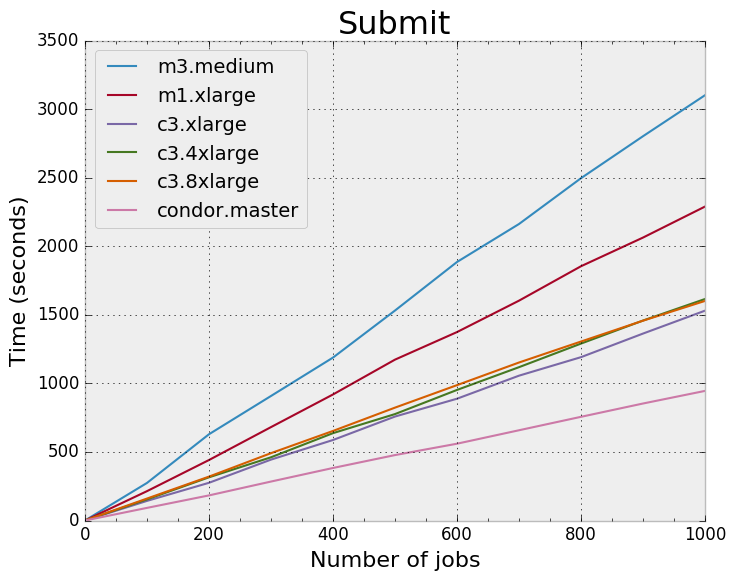
\includegraphics[width=1\linewidth]{GridScaleSubmit.png}}
	\endminipage \vfill
	\minipage{0.49\textwidth}
		\subfloat[][]{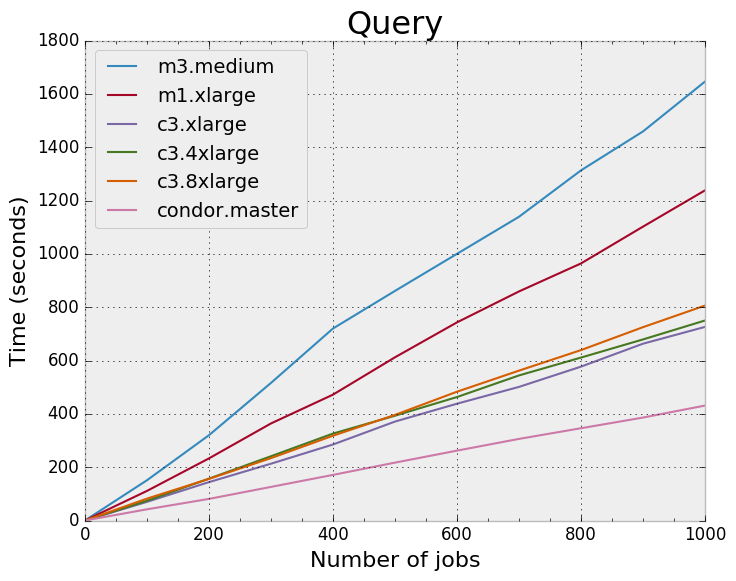
\includegraphics[width=1\linewidth]{GridScaleQuery.png}}
	\endminipage \hfill
	\minipage{0.49\textwidth}
		\subfloat[][]{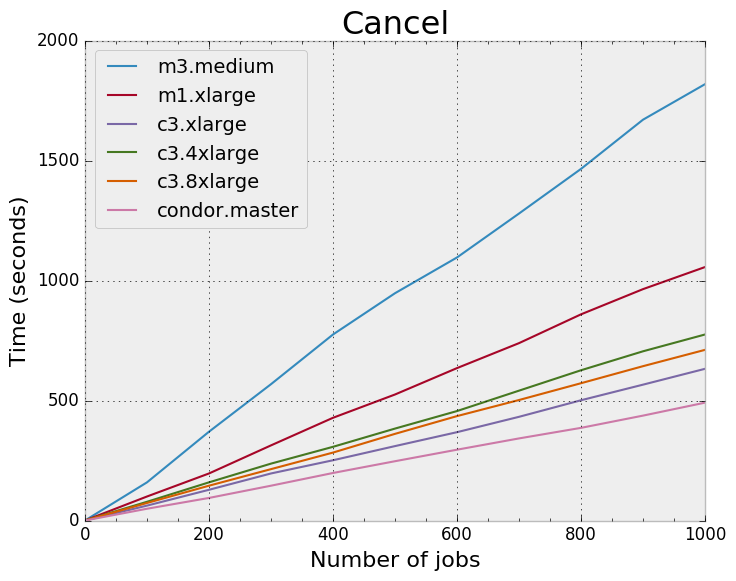
\includegraphics[width=1\linewidth]{GridScaleCancel.png}}
	\endminipage \hfill
	\caption{Comparison for submission, query and cancellation times in the case of only one session per SSH connection.}
	\label{SingleSession}
\end{figure}

While the \verb|m3.medium| clearly lags behind given its low bandwidth, the three high-CPU \verb|c3| instances exhibit close performance and are faster than the high-throughput \verb|m1.xlarge| instance, indicating that bandwidth only has diminishing returns and the CPU is more important, while latency remains a constant factor.


When connections to master nodes are allowed to open multiple sessions, Figure \ref{MultiSession}  shows the rate of commands per second improves dramatically across the board. For each of the three commands, multi-session SSH connections bring 15x improvements to the execution time. The \verb|c3| instances continue to exhibit similar performance, which is mildly surprising due to the vastly superior specifications of the \verb|c3.8xlarge| instance.

\begin{figure}[h]
	\centering
	\minipage{0.49\textwidth}
		\subfloat[][]{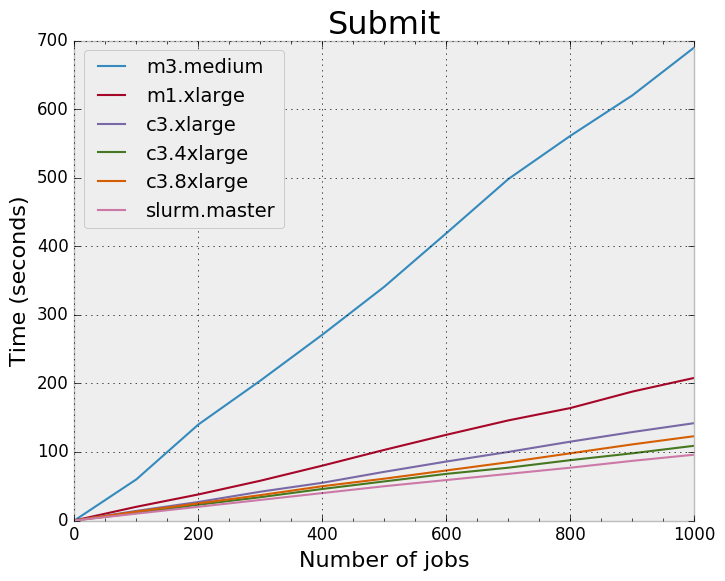
\includegraphics[width=1\linewidth]{GridScaleSubmitAsync.png}}
	\endminipage \vfill
	\minipage{0.49\textwidth}
		\subfloat[][]{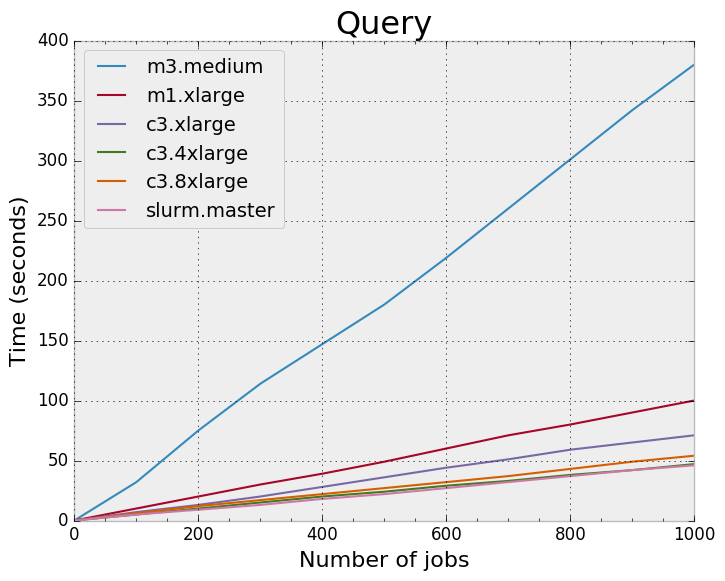
\includegraphics[width=1\linewidth]{GridScaleQueryAsync.png}}
	\endminipage \hfill
	\minipage{0.49\textwidth}
		\subfloat[][]{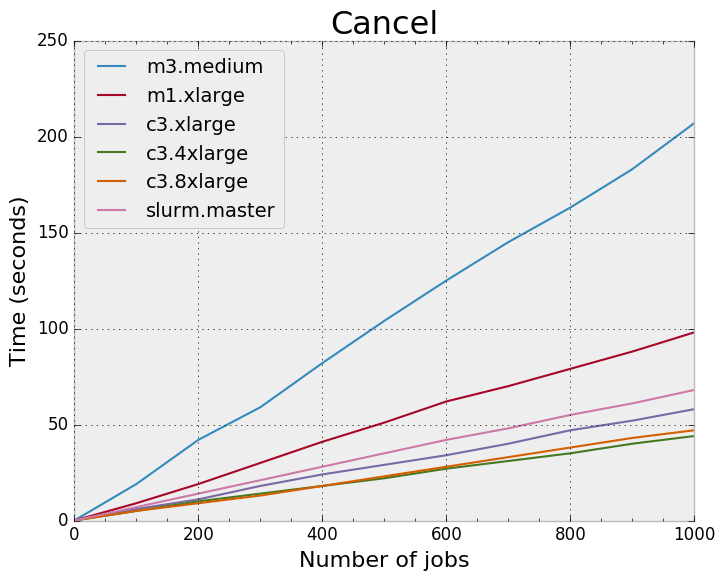
\includegraphics[width=1\linewidth]{GridScaleCancelAsync.png}}
	\endminipage \hfill
	\caption{Comparison for submission, query and cancellation times in the case of multiple sessions per SSH connection.}
	\label{MultiSession}
\end{figure}

In this case, we are comparing the command latencies with the Slurm master node, which has the same characteristics as the HTCondor one. Despite being on the local network when the benchmark was run, it responds to \textit{cancel} requests slower than the \verb|c3| instances.

\section{OpenMOLE Workflow Benchmarks}

On the OpenMOLE level, we are interested in how the application behaves as a whole when distributing real algorithms over a cloud cluster. In this section, we look at the performance of the system when engaged in running two full different workflows with different underlying cluster configurations. We then estimate the cost of running each of the workflows.

\subsection{$\pi$ Computation}

The algorithm presented in Appendix \ref{Pi}, Listing \ref{PiComputation} computes a Monte-Carlo estimation of $\pi$. It first computes the result of 100 parallel executions of the \verb|ScalaTask| starting each time from a generated random seed, after which it collects the results and averages them to give a final estimation. This is still a simple algorithm, but more substantial than the ones we have presented so far.

Table \ref{PiTable} summarises the results of running the algorithm 10 times with different types of master and worker nodes, while also using different number of estimations to obtain the final result. Note that each estimation corresponds to a random seed in the workflow. The total cost of each run is computed using the prices in Table \ref{InstancePrices} and we also show prices for on-demand cluster, even if all the experiments were carried out using full spot clusters.

\begin{table}[h]
\centering
\begin{adjustbox}{width=1\textwidth}
\begin{tabular}{cccccccc}
 &  &  &  &  &  & \multicolumn{2}{c}{\textbf{Total Price (\$)}} \\ \cline{7-8} 
\textbf{} & \textbf{Master Instance} & \textbf{Worker Instance} & \textbf{Worker Nodes} & \textbf{Estimations} & \multicolumn{1}{c|}{\textbf{Time (s)}} & \multicolumn{1}{c|}{\textbf{Spot}} & \multicolumn{1}{c|}{\textbf{On-Demand}} \\ \cline{2-8} 
\multicolumn{1}{c|}{1} & \multicolumn{1}{c|}{m1.medium} & \multicolumn{1}{c|}{m1.small} & \multicolumn{1}{c|}{1} & \multicolumn{1}{c|}{200} & \multicolumn{1}{c|}{5054} & \multicolumn{1}{c|}{0.04} & \multicolumn{1}{c|}{0.284} \\ \cline{2-8} 
\multicolumn{1}{c|}{2} & \multicolumn{1}{c|}{c1.medium} & \multicolumn{1}{c|}{m1.small} & \multicolumn{1}{c|}{1} & \multicolumn{1}{c|}{100} & \multicolumn{1}{c|}{3565} & \multicolumn{1}{c|}{0.02} & \multicolumn{1}{c|}{0.142} \\ \cline{2-8} 
\multicolumn{1}{c|}{3} & \multicolumn{1}{c|}{c3.8xlarge} & \multicolumn{1}{c|}{c3.xlarge} & \multicolumn{1}{c|}{4} & \multicolumn{1}{c|}{100} & \multicolumn{1}{c|}{929} & \multicolumn{1}{c|}{0.499} & \multicolumn{1}{c|}{2.862} \\ \cline{2-8} 
\multicolumn{1}{c|}{4} & \multicolumn{1}{c|}{c3.8xlarge} & \multicolumn{1}{c|}{c3.xlarge} & \multicolumn{1}{c|}{8} & \multicolumn{1}{c|}{100} & \multicolumn{1}{c|}{1032} & \multicolumn{1}{c|}{0.671} & \multicolumn{1}{c|}{3.818} \\ \cline{2-8} 
\multicolumn{1}{c|}{5} & \multicolumn{1}{c|}{c3.8xlarge} & \multicolumn{1}{c|}{c3.xlarge} & \multicolumn{1}{c|}{8} & \multicolumn{1}{c|}{100} & \multicolumn{1}{c|}{915} & \multicolumn{1}{c|}{0.671} & \multicolumn{1}{c|}{3.818} \\ \cline{2-8} 
\multicolumn{1}{c|}{6} & \multicolumn{1}{c|}{c3.8xlarge} & \multicolumn{1}{c|}{c3.xlarge} & \multicolumn{1}{c|}{8} & \multicolumn{1}{c|}{100} & \multicolumn{1}{c|}{2820} & \multicolumn{1}{c|}{0.671} & \multicolumn{1}{c|}{3.818} \\ \cline{2-8} 
\multicolumn{1}{c|}{7} & \multicolumn{1}{c|}{c3.8xlarge} & \multicolumn{1}{c|}{c3.xlarge} & \multicolumn{1}{c|}{16} & \multicolumn{1}{c|}{100} & \multicolumn{1}{c|}{792} & \multicolumn{1}{c|}{1.015} & \multicolumn{1}{c|}{5.73} \\ \cline{2-8} 
\multicolumn{1}{c|}{8} & \multicolumn{1}{c|}{c3.4xlarge} & \multicolumn{1}{c|}{c3.xlarge} & \multicolumn{1}{c|}{4} & \multicolumn{1}{c|}{100} & \multicolumn{1}{c|}{1142} & \multicolumn{1}{c|}{0.34} & \multicolumn{1}{c|}{1.909} \\ \cline{2-8} 
\multicolumn{1}{c|}{9} & \multicolumn{1}{c|}{c3.4xlarge} & \multicolumn{1}{c|}{c3.xlarge} & \multicolumn{1}{c|}{8} & \multicolumn{1}{c|}{100} & \multicolumn{1}{c|}{964} & \multicolumn{1}{c|}{0.512} & \multicolumn{1}{c|}{2.865} \\ \cline{2-8} 
\multicolumn{1}{c|}{10} & \multicolumn{1}{c|}{c3.4xlarge} & \multicolumn{1}{c|}{c3.xlarge} & \multicolumn{1}{c|}{16} & \multicolumn{1}{c|}{1000} & \multicolumn{1}{c|}{4827} & \multicolumn{1}{c|}{1.712} & \multicolumn{1}{c|}{9.554} \\ \cline{2-8} 
\end{tabular}
\end{adjustbox}
\caption{Summary of various runs of the $\pi$ computation algorithm, including the price of each execution.}
\label{PiTable}
\end{table}

We can already observe large differences in execution times between runs with similar cluster configurations. For example, run 6 is over 300\% slower than run 5, given identical instance types and the same number of jobs. By inspecting the load of the system during the workflow run, we observed that the available CPU and memory often fluctuated aggressively without the instances being flooded with requests. We partially attribute this to the fact that in the end we are working with virtual instances that share the same physical machine.

Very long runs like 7 occur occasionally when instances in the cluster are not reliable. An occasional pattern occurring in particular with spot clusters was instances rejecting to receive jobs due to insufficient disk space, although we are not storing anything specifically on the machines themselves and the working directory is always set to \verb|/home|, the volume shared on the network by StarCluster.

Since each run spends the first approximately 330 - 380 seconds setting up the cluster, we consider total running times of about 1000 seconds acceptable. This is because the simple task executions used here actually require the same networking resources as genuinely CPU-intensive ones to reach their destinations execution nodes, so more complicated workflows are not necessarily more time-consuming.

\subsection{Random Forest}

The random forest workflow in Appendix \ref{Forest}, Figure \ref{RandomForest} explores the parameters of the \verb|forest.py| script, which performs random forest image classification \cite{RandFor} to distinguish 3 types of leaves. The Python script is packaged as a CARE task and receives as parameters the location of the dataset, the number of trees in a forest and the depth of each tree. The output of the script is a single floating point number representing the precision of the k-fold trained classifier.

As before, we ran the workflow multiple times with different configurations, but eventually only chose the results in Table \ref{ForestTable} for display.

\begin{table}[h]
\centering
\begin{adjustbox}{width=1\textwidth}
\begin{tabular}{cccccccc}
 &  &  &  &  &  & \multicolumn{2}{c}{\textbf{Total Price (\$)}} \\ \cline{7-8} 
\textbf{} & \textbf{Master Instance} & \textbf{Worker Instance} & \textbf{Worker Nodes} & \textbf{Generated Jobs} & \multicolumn{1}{c|}{\textbf{Time (s)}} & \multicolumn{1}{c|}{\textbf{Spot}} & \multicolumn{1}{c|}{\textbf{On-Demand}} \\ \cline{2-8} 
\multicolumn{1}{c|}{1} & \multicolumn{1}{c|}{c3.8xlarge} & \multicolumn{1}{c|}{c3.xlarge} & \multicolumn{1}{c|}{4} & \multicolumn{1}{c|}{337} & \multicolumn{1}{c|}{3219} & \multicolumn{1}{c|}{0.499} & \multicolumn{1}{c|}{2.862} \\ \cline{2-8} 
\multicolumn{1}{c|}{2} & \multicolumn{1}{c|}{c3.8xlarge} & \multicolumn{1}{c|}{c3.xlarge} & \multicolumn{1}{c|}{8} & \multicolumn{1}{c|}{337} & \multicolumn{1}{c|}{2625} & \multicolumn{1}{c|}{0.671} & \multicolumn{1}{c|}{3.818} \\ \cline{2-8} 
\multicolumn{1}{c|}{3} & \multicolumn{1}{c|}{c3.4xlarge} & \multicolumn{1}{c|}{c3.xlarge} & \multicolumn{1}{c|}{8} & \multicolumn{1}{c|}{337} & \multicolumn{1}{c|}{4117} & \multicolumn{1}{c|}{1.024} & \multicolumn{1}{c|}{5.73} \\ \cline{2-8} 
\end{tabular}
\end{adjustbox}
\caption{Summary of various runs of the random forest classifier training, including the price of each execution.}
\label{ForestTable}
\end{table}

Here we can notice that, despite only having 337 generated jobs to execute, the tasks were indeed more time consuming, which is in accordance with the training of the classifier in the Python script. It would probably be expected that the second cluster configuration is the fastest one, but it is interesting to compare run 1 and 3. This leads us to the conclusion that a powerful instance as the master is indicated to having a larger pool of workers, since the master can easily become a bottleneck for very demanding workflows.

\section{Spot Clusters}

Throughout this section, we have learned that clusters consisting entirely of spot instances are not always reliable. Although we can deal with instances being revoked by EC2 via OpenMOLE's resubmission mechanisms, this has only been necessary once  during the whole development and testing process. 

Spot prices do not usually change abruptly, so instances being suddenly revoked is not a very common problem. Additionally OpenMOLE can already recover from sudden job failures and non-critical instances failing.

However, we do not recommend ever letting the master node of a cluster be a spot instance, since it being revoked would result into an irrecuperable state for OpenMOLE. Apart from the possibility of it being revoked, the biggest concern is in fact the potential flakiness of spot instances. Theoretically, spots are advertised as being the same as on-demand instances, but in practice we have found them to be more unreliable.

Despite all the potential issues with spot instances, we do recognize that they offer great value and workflows run on spot clusters are, as seen in Table \ref{PiTable}, on average between 5 and 8 times cheaper than on-demand clusters. This is particularly true if generating many short-lived jobs whose recovery in case of failure is cheap.

Another issue discovered during the evaluation was that Amazon limits by default the number of spot instances a user can bid for or run simultaneously to 20. This is, however, not a hard requirement and can be changed by negotiating directly with the provider.

\section{Challenges and Limitations}

The evaluation of our implementation on both the OpenMOLE and the GridScale level was influenced by several factors. We did manage to overcome some of the problems, while others issues require deeper changes in the structure of the project in order to be solved.

One of the main drawbacks of our evaluation process was that it required extensive manual intervention and supervision. Although we were able to write a framework that automatically collects data about job submission statistics as part of GridScale, the holistic evaluation at the OpenMOLE layer was mostly performed using either the console mode of the command line tool or the web interface. This did not provide us with too much control over testing scenarios and we were limited to running the application as a simple user. More granular access to the internals of the application would have enabled us to more easily identify bottlenecks.

A challenge adjacent to the first point we made was the lack of integration testing present in both GridScale and OpenMOLE. Although setting up an integration testing framework is an inherently hard problem in the context of applications dealing with distributed systems, the presence of a reliable test suite would certainly increase the confidence of the developers in the functional correctness of the product and eventually speed up development cycles.

One of the reasons for which the experiment results may be seriously skewed is the volatility of Amazon's EC2 resource pool. Especially in the case of spot instances, which we have used almost exclusively for experiments, differences in performance can become a rather serious problem when trying to diagnose issues with the application.

Our comparison with job submission systems supported by the Department of Computing may also suffer from inaccuracies. In fact, this is a more general problem, since comparing systems relying on different resource pools will always cause slight differences. One concrete example is the comparison between workflows run on an EC2 cluster and on DoC's Slurm or HTCondor deployment. The average machine in the department is the rough equivalent of the \verb|c3.4xlarge|, the second most powerful machine we rented for testing purposes. The network speed of the local connection also generally skews results against the cloud approach, although we always accounted for it when trying to explain performance differences.